% ---------------------------------------------------------------------------------------
% TP1, DCC831 (UFMG): two-page extended summary in the ISMIR 2026 template.
% Topic: Undertale-style game music with Markov chains (Bach chorales only validate the implementation).
%
% Compile:  latexmk -pdf ismir_summary.tex      (or pdflatex + bibtex + pdflatex x2)
% Numbers in the text, Table 1 and Figure 1 are generated by make_figures.py
% (numbers.tex, results_table.tex, figs/novelty.pdf). Do not edit them by hand.
% ---------------------------------------------------------------------------------------
\documentclass{article}
\usepackage[T1]{fontenc}
\usepackage[utf8]{inputenc}

% Layout switch: true  -> anonymous "submission" layout (line numbers, no author names)
%                false -> author names printed (used for the course submission)
\newif\ifsubmissionlayout
\submissionlayoutfalse
\ifsubmissionlayout\usepackage[submission]{ismir}\else\usepackage{ismir}\fi

\usepackage{amsmath,cite,url}
\usepackage{graphicx}
\urlstyle{sf}                       % Courier is not available everywhere; sans-serif, like the software names

% Gerado por paper/make_figures.py a partir de docs/*.csv. NÃO edite à mão.
\newcommand{\bachCorpusPar}{0.20}
\newcommand{\bachMelodyFiveCov}{68}
\newcommand{\bachMelodyFivePhr}{86}
\newcommand{\bachMelodyFourCov}{73}
\newcommand{\bachMelodyFourPhr}{64}
\newcommand{\bachMelodyOneCov}{99}
\newcommand{\bachMelodyOnePhr}{1}
\newcommand{\bachMelodyThreeCov}{82}
\newcommand{\bachMelodyThreePhr}{30}
\newcommand{\bachMelodyTwoCov}{93}
\newcommand{\bachMelodyTwoPhr}{5}
\newcommand{\bachSatbFourCov}{32}
\newcommand{\bachSatbFourPar}{0.24}
\newcommand{\bachSatbFourPhr}{89}
\newcommand{\bachSatbOneCov}{60}
\newcommand{\bachSatbOnePar}{0.19}
\newcommand{\bachSatbOnePhr}{6}
\newcommand{\bachSatbThreeCov}{34}
\newcommand{\bachSatbThreePar}{0.21}
\newcommand{\bachSatbThreePhr}{74}
\newcommand{\bachSatbTwoCov}{41}
\newcommand{\bachSatbTwoPar}{0.17}
\newcommand{\bachSatbTwoPhr}{45}
\newcommand{\utMelodyFourCov}{17}
\newcommand{\utMelodyFourFeas}{20}
\newcommand{\utMelodyFourRem}{n/a}
\newcommand{\utMelodyFourSec}{79}
\newcommand{\utMelodyFourWin}{97}
\newcommand{\utMelodyOneCov}{73}
\newcommand{\utMelodyOneFeas}{20}
\newcommand{\utMelodyOneRem}{6}
\newcommand{\utMelodyOneSec}{15}
\newcommand{\utMelodyOneWin}{8}
\newcommand{\utMelodyThreeCov}{21}
\newcommand{\utMelodyThreeFeas}{20}
\newcommand{\utMelodyThreeRem}{27}
\newcommand{\utMelodyThreeSec}{69}
\newcommand{\utMelodyThreeWin}{91}
\newcommand{\utMelodyTwoCov}{33}
\newcommand{\utMelodyTwoFeas}{20}
\newcommand{\utMelodyTwoRem}{17}
\newcommand{\utMelodyTwoSec}{48}
\newcommand{\utMelodyTwoWin}{68}
\newcommand{\utOuterFourCov}{7}
\newcommand{\utOuterFourFeas}{0}
\newcommand{\utOuterFourRem}{n/a}
\newcommand{\utOuterFourSec}{78}
\newcommand{\utOuterFourWin}{98}
\newcommand{\utOuterOneCov}{28}
\newcommand{\utOuterOneFeas}{20}
\newcommand{\utOuterOneRem}{11}
\newcommand{\utOuterOneSec}{32}
\newcommand{\utOuterOneWin}{46}
\newcommand{\utOuterThreeCov}{8}
\newcommand{\utOuterThreeFeas}{0}
\newcommand{\utOuterThreeRem}{n/a}
\newcommand{\utOuterThreeSec}{68}
\newcommand{\utOuterThreeWin}{96}
\newcommand{\utOuterTwoCov}{9}
\newcommand{\utOuterTwoFeas}{20}
\newcommand{\utOuterTwoRem}{22}
\newcommand{\utOuterTwoSec}{60}
\newcommand{\utOuterTwoWin}{89}
\newcommand{\utPianoFourCov}{5}
\newcommand{\utPianoFourFeas}{0}
\newcommand{\utPianoFourRem}{n/a}
\newcommand{\utPianoFourSec}{78}
\newcommand{\utPianoFourWin}{100}
\newcommand{\utPianoOneCov}{19}
\newcommand{\utPianoOneFeas}{20}
\newcommand{\utPianoOneRem}{18}
\newcommand{\utPianoOneSec}{49}
\newcommand{\utPianoOneWin}{76}
\newcommand{\utPianoThreeCov}{6}
\newcommand{\utPianoThreeFeas}{0}
\newcommand{\utPianoThreeRem}{n/a}
\newcommand{\utPianoThreeSec}{75}
\newcommand{\utPianoThreeWin}{99}
\newcommand{\utPianoTwoCov}{6}
\newcommand{\utPianoTwoFeas}{0}
\newcommand{\utPianoTwoRem}{n/a}
\newcommand{\utPianoTwoSec}{77}
\newcommand{\utPianoTwoWin}{98}
                 % \utPianoOneWin, \bachCorpusPar, ... (generated)

\title{Undertale-Style Game Music with Markov Chains: Order, Memorization and Anti-Plagiarism}

\oneauthor
  {Samuel Lucca Viana Miranda (2022043566)}
  {Departamento de Ci\^encia da Computa\c{c}\~ao, UFMG}
\def\authorname{Samuel Lucca Viana Miranda}

\sloppy % please retain sloppy command for improved formatting

\begin{document}

\maketitle

\begin{abstract}
We present a symbolic generator of video-game music based on order-$n$ Markov chains trained on 110 fan-made piano transcriptions of the \textsf{UNDERTALE} soundtrack. A state is a sonority (bar position, sounding pitches, articulation, duration), and a piece is a loop of 4-bar sections following a form such as AABA. Bach chorales serve only to validate the implementation of the Markov model; the proposed system targets game music. Without protection, the full-piano chain of order~1 copies \utPianoOneWin\% of its 6-event windows, whereas the melody-only chain of order~1 copies just \utMelodyOneSec\% of its sections. A rejection-based anti-plagiarism constraint makes the order-1 piano chain usable in \utPianoOneFeas{} of 20 seeds with \utPianoOneRem\% of windows still copied, yielding collages of fragments from different songs. Code, MIDI and audio are in the repository at \url{https://github.com/Samuel-Wisart/Generative_Markov_Undertale_Music}; the corpus is not distributed.
\end{abstract}

\section{Introduction}\label{sec:introduction}

Video-game soundtracks are short, loop-based and built on identifiable motives, which suits Markov models: the next state is sampled from a distribution over the last $n$ states, counted from a corpus \cite{Hiller59,Ames89}. The same properties make memorization a risk, since a high order reproduces long fragments of the corpus \cite{Pachet03,Papadopoulos14}, which matters for originality and copyright. We build a generator of \emph{Undertale}-style music \cite{Fox15} (piano texture, 4/4, 4-bar sections, loop forms such as AABA) and quantify how order, texture and an anti-plagiarism constraint trade novelty against fidelity. Bach chorales are used only as a test bed to validate the Markov implementation (Section~\ref{sec:results}).

\section{Related Work}\label{sec:related}

Markov composition dates back to the \emph{Illiac Suite} \cite{Hiller59} (survey: \cite{Ames89}). The Continuator uses variable-order models \cite{Pachet03}; Markov constraints make generation steerable \cite{PachetRoy11}, and Papadopoulos et al.\ \cite{Papadopoulos14} avoid plagiarism by bounding verbatim copies, of which our \textsf{max-copy} rule is a simpler section-level variant. Game music has symbolic datasets such as NES-MDB \cite{Donahue18} and VGMIDI, 823 piano arrangements of game soundtracks \cite{Ferreira19}, close to our corpus. We study a deliberately simple, exactly measurable Markov baseline.

% The two wide floats are declared here, on page 1, so that they can sit at the top of page 2
% (a two-column float can only be placed on a page after the one where it is declared).
\begin{table*}
  \centering
  \footnotesize
  \renewcommand{\arraystretch}{0.95}
  \setlength{\tabcolsep}{4.5pt}
  \begin{tabular}{|l|c|r|c|c|c|c|c|}
    \hline
    Texture & $n$ & Contexts & Coverage (\%) & Copied windows (\%) & Copied sections (\%) & \multicolumn{2}{c|}{With $\tau=0.3$: feasible / copied (\%)} \\ \hline
    Melody & 1 & 2{,}450 & 73 & 8 & 15 & 20/20 & 6 \\
 & 2 & 5{,}373 & 33 & 68 & 48 & 20/20 & 17 \\
 & 3 & 6{,}337 & 21 & 91 & 69 & 20/20 & 27 \\
 & 4 & 6{,}808 & 17 & 97 & 79 & 20/20 & n/a \\
\hline
Melody+bass & 1 & 8{,}304 & 28 & 46 & 32 & 20/20 & 11 \\
 & 2 & 10{,}816 & 9 & 89 & 60 & 20/20 & 22 \\
 & 3 & 11{,}556 & 8 & 96 & 68 & 0/20 & n/a \\
 & 4 & 12{,}067 & 7 & 98 & 78 & 0/20 & n/a \\
\hline
Piano & 1 & 10{,}077 & 19 & 76 & 49 & 20/20 & 18 \\
 & 2 & 12{,}036 & 6 & 98 & 77 & 0/20 & n/a \\
 & 3 & 12{,}681 & 6 & 99 & 75 & 0/20 & n/a \\
 & 4 & 13{,}128 & 5 & 100 & 78 & 0/20 & n/a \\ \hline
  \end{tabular}
  \caption{Effect of the order $n$ on the Undertale corpus (60 ABCD pieces per row). \emph{Coverage}: contexts of unseen pieces found in training (5-fold cross-validation by piece). \emph{Copied}: windows ($k=8$ for melody and melody+bass, $k=6$ for piano) and whole sections found verbatim in the corpus. With $\tau=0.3$: seeds (of 20) that worked, and copying left (``n/a'': infeasible, or no full window).}
  \label{tab:results}
\end{table*}

\begin{figure*}
  \centering
  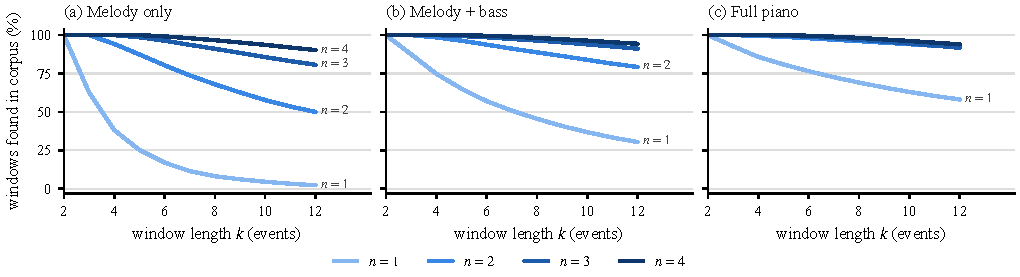
\includegraphics[width=0.92\textwidth]{figs/novelty.pdf}
  \caption{Novelty curves on the Undertale corpus: share of generated windows of length $k$ found verbatim in the corpus. Windows up to $n{+}1$ events are corpus fragments by construction; where a curve leaves 100\% marks the novelty horizon.}
  \label{fig:novelty}
\end{figure*}

\section{Method}\label{sec:method}

\subsection{Corpus and Representation}

The corpus has 110 fan-made MIDI piano transcriptions of the \textsf{UNDERTALE} soundtrack (not distributed). Discarding 10 files with changing meter and 3 almost empty ones leaves 97; the 80 with four-beat bars yield 1{,}115 sections of four bars. Notes are read with \textsf{music21} \cite{Cuthbert10} and quantized to 12 ticks per quarter note. Each piece is transposed, using the Krumhansl-Schmuckler key estimate \cite{Krumhansl90}, to the white-key collection of its relative C major / A minor, so major and minor pieces share one vocabulary.

A \emph{state} is a slice of the score, $e=(b,\mathbf{p},\mathbf{a},d)$: bar position $b$, sorted sounding pitches $\mathbf{p}$ (empty for a rest), attack flags $\mathbf{a}$ and duration $d$. Slices start at each onset and at real rests (at least a third of a beat); smaller articulation gaps are absorbed by the previous note. We compare three textures: \emph{melody} (highest note, G3 and above), \emph{melody+bass} (highest and lowest notes) and full \emph{piano}.

\subsection{Markov Model}

An order-$n$ chain estimates, by counting over sections,
\begin{equation}\label{eq:markov}
P(e_t \mid e_{t-n},\ldots,e_{t-1}) = \frac{c(e_{t-n},\ldots,e_t)}{c(e_{t-n},\ldots,e_{t-1})}.
\end{equation}
Each section is padded with $n$ start symbols and closed by an end marker, so the chain learns when to stop. There is no smoothing; sampling uses $p\propto c^{1/T}$ with temperature $T$.

\subsection{Generation and Constraints}

A piece follows a form (AABA by default): each distinct letter is a section sampled from the chain, and repeated letters repeat it, as in game loops. A section is accepted only if (i) it ends with the end marker and lasts exactly four bars, (ii) it is not silent, and (iii) optionally, at most a fraction $\tau$ of its windows of $k$ consecutive events occur verbatim in the corpus ($k=8$ for melody and melody+bass, $k=6$ for piano). MIDI is written with \textsf{music21}; a simple synthesizer (piano or chiptune timbre) renders audio for listening only.

\section{Experiments and Results}\label{sec:results}

\textbf{Validation on Bach chorales.} The implementation was first checked on the 307 four-voice 4/4 chorales of \textsf{music21} \cite{Cuthbert10}. The chain, sampling and rejection loop are the same code; only the corpus reader and phrase rules (fermatas, final tonic) are chorale-specific. The expected behavior was observed: pieces use only transitions present in the counts, phrases join metrically and end on the tonic, memorization grows with the order (whole-phrase copies from \bachMelodyOnePhr\% to \bachMelodyFivePhr\% for melody orders 1 to 5, and from \bachSatbOnePhr\% to \bachSatbFourPhr\% for four voices at orders 1 to 4), and parallel fifths and octaves stay between \bachSatbTwoPar{} and \bachSatbFourPar{} per 100 transitions against \bachCorpusPar{} in the chorales. These pieces are not part of the proposed system.

\textbf{Memorization} (\tabref{tab:results}). Songs share little vocabulary: for an unseen piece only \utPianoOneCov\% of the order-1 piano contexts exist in training (\bachSatbOneCov\% for Bach), so the chain mostly recites the song it enters. Unprotected, the order-1 piano chain copies \utPianoOneWin\% of its windows and \utPianoOneSec\% of its sections; melody+bass copies \utOuterOneWin\% and \utOuterOneSec\%. Only the melody chain of order 1 is mostly original (\utMelodyOneWin\% and \utMelodyOneSec\%), at the price of coherence: an order-1 chain only guarantees pairs of consecutive notes (\figref{fig:novelty}).

\textbf{Anti-plagiarism.} With $\tau=0.3$ the order-1 piano chain works in \utPianoOneFeas{} of 20 seeds with \utPianoOneRem\% of windows still copied, as do melody+bass orders 1 and 2 and melody orders 1 to 4; higher orders are infeasible (0 of 20) because the chain is almost deterministic. Defaults: melody $n=2$, melody+bass and piano $n=1$, all with $\tau=0.3$.

\textbf{Examples.} We rendered ten pieces. With $\tau=0.3$, seven copy between 8 and 24\% of their windows (these are in the repository); without it, order-1 piano seeds 1 to 3 copy 14, 100 and 100\% (not distributed).

\section{Discussion and Future Work}\label{sec:discussion}

The chain has no global plan beyond the section loop. The corpus is small, made of fan transcriptions of uneven quality, and each song has its own vocabulary, which explains the strong memorization. The evaluation is objective, without a listening study. A relative (interval-based) representation should recombine material across songs more freely; other extensions are a melody chain with a conditioned harmonization model \cite{Allan05}, variable-order models with back-off \cite{Pachet03}, and listening tests.

\section{AI Usage Statement}

The software and the first draft of this manuscript were produced with the assistance of Claude Code (Anthropic, model Claude Sonnet 5.5) with help in the implementation and answering questions about the algorithms and getting references.

\section{Ethics Statement}

The corpus consists of fan transcriptions of copyrighted music \cite{Fox15}, used for study only and not distributed. Copy rates do not prove originality, so only pieces generated with the anti-plagiarism constraint are released.

\bibliography{references}

\end{document}
